%%
%% This is file `sample-sigconf.tex',
%% generated with the docstrip utility.
%%
%% The original source files were:
%%
%% samples.dtx  (with options: `sigconf')
%% 
%% IMPORTANT NOTICE:
%% 
%% For the copyright see the source file.
%% 
%% Any modified versions of this file must be renamed
%% with new filenames distinct from sample-sigconf.tex.
%% 
%% For distribution of the original source see the terms
%% for copying and modification in the file samples.dtx.
%% 
%% This generated file may be distributed as long as the
%% original source files, as listed above, are part of the
%% same distribution. (The sources need not necessarily be
%% in the same archive or directory.)
%%
%% The first command in your LaTeX source must be the \documentclass command.
\documentclass[sigconf]{acmart}
\settopmatter{printacmref=false} % Removes citation information below abstract
\renewcommand\footnotetextcopyrightpermission[1]{} % removes footnote with conference information in first column
\pagestyle{plain} % removes running headers

%%
%% \BibTeX command to typeset BibTeX logo in the docs
\AtBeginDocument{%
  \providecommand\BibTeX{{%
    \normalfont B\kern-0.5em{\scshape i\kern-0.25em b}\kern-0.8em\TeX}}}

%% Rights management information.  This information is sent to you
%% when you complete the rights form.  These commands have SAMPLE
%% values in them; it is your responsibility as an author to replace
%% the commands and values with those provided to you when you
%% complete the rights form.






%%
%% Submission ID.
%% Use this when submitting an article to a sponsored event. You'll
%% receive a unique submission ID from the organizers
%% of the event, and this ID should be used as the parameter to this command.
%%\acmSubmissionID{123-A56-BU3}

%%
%% The majority of ACM publications use numbered citations and
%% references.  The command \citestyle{authoryear} switches to the
%% "author year" style.
%%
%% If you are preparing content for an event
%% sponsored by ACM SIGGRAPH, you must use the "author year" style of
%% citations and references.
%% Uncommenting
%% the next command will enable that style.
%%\citestyle{acmauthoryear}

%%
%% end of the preamble, start of the body of the document source.
\begin{document}

%%
%% The "title" command has an optional parameter,
%% allowing the author to define a "short title" to be used in page headers.
\title{Privacy Implications of Smart Wearable Devices}

%%
%% The "author" command and its associated commands are used to define
%% the authors and their affiliations.
%% Of note is the shared affiliation of the first two authors, and the
%% "authornote" and "authornotemark" commands
%% used to denote shared contribution to the research.
\author{Gautam Worah}
\email{gworah@ncsu.edu}
\affiliation{%
  \institution{North Carolina State University}
}

\author{Jubeen Shah}
\email{jnshah2@ncsu.edu}
\affiliation{%
  \institution{North Carolina State University}
}


\author{Sujal}
\email{ssujal@ncsu.edu}
\affiliation{%
  \institution{North Carolina State University}
}



%%
%% By default, the full list of authors will be used in the page
%% headers. Often, this list is too long, and will overlap
%% other information printed in the page headers. This command allows
%% the author to define a more concise list
%% of authors' names for this purpose.


%%
%% The abstract is a short summary of the work to be presented in the
%% article.
\begin{abstract} \label{abstract}
 Wearable Technology refers to the category of gadgets worn by the user to provide user-specific information to the device it pairs. Wearables have become popular in several high-impact domains such as healthcare, security, and entertainment. 

Wearables are essentially sensor nodes collecting data for the master server (the smartphone). Smartwatches, glasses, clothing, and even jewelry are some of the examples. On the one hand, they provide the opportunity to enhance efficiency across industries by continuously monitoring human activity. However, they also pose security concerns in comparison to other computing devices, because these wearable technologies are so much more personal. The amount and type of data collected by these devices may be used to reveal one’s identity, and therefore security challenges are critical to their usage. Thus, the primary goal of this project is to identify what are the privacy concerns of users, how they perceive the data collection, and what is their level of awareness with regards to the data usage and privacy policies of these devices. 

We studied the implications caused by a broad category of these devices, in terms of security and privacy vulnerabilities. We discuss the various types of data collected, the frequency of data collection, and the privacy risks posed by them based on the kind of wearable used in this paper.
\end{abstract}

%%
%% The code below is generated by the tool at http://dl.acm.org/ccs.cfm.
%% Please copy and paste the code instead of the example below.
%%


%%
%% Keywords. The author(s) should pick words that accurately describe
%% the work being presented. Separate the keywords with commas.
\keywords{Privacy, Wearable computing, Wearable devices, Form factors, Privacy concerns, User studies, Human factors}


%%
%% This command processes the author and affiliation and title
%% information and builds the first part of the formatted document.
\maketitle

\section{Description and motivation} \label{motivation}
As noted in the abstract The ability of smart wearables to ubiquitously and continuously collect and transmit data to their sister devices (smartphones, other IoT devices) poses many privacy risks \cite{Paul:2014:PIW:2659651.2659683}. Their sensitive nature accentuates these privacy risks as they can often reveal vital information about an individual’s health, their daily routine, and the people they interact with. Moreover, since the mass adoption of these devices is recent, most users are still unaware of the potential implications of continuous monitoring, storage, profiling, and analysis of health and personal data \cite{10.1007/978-3-662-48051-9_17}. 

The answers to the questions regarding user awareness, privacy concerns, and perception of data collection methodologies helped us understand what the current mentality of users in the context of smart wearable privacy is. Also, it helps us understand their level of understanding concerning the types and extent of data that can be collected and what would be the best means to educate them to protect their sensitive information is.

In section \textbf{\ref{literatureReview}} we will discuss about the the literature reviewed, followed by the approach we followed in section \textbf{\ref{approach}}. Then we will proceed to describing the study design in brief in section \textbf{\ref{studyDesign}}. We would then discuss the results from survey in section \textbf{\ref{appleAnalysis}}, \textbf{\ref{snapchatAnalysis}}, and \textbf{\ref{levisAnalysis}}. Finally we describe the limitations and future work of the project in Section \textbf{\ref{limitationAndFutureWork}}.

\section{Literature Review} \label{literatureReview}

Privacy and security concerns have been discussed for a long time, but the implications concerning wearable devices are still relatively new \cite{Mancini:2009:SPE:1620545.1620547}. In general, smart devices continuously collect data via sensors, and their intricate designs accrue various challenges in providing user privacy. Although many studies have been focused on mobile devices, and applications, there is still a vast scope in understanding the privacy behaviors of wearable technology\cite{TROSHYNSKI2011}\cite{Hoyle:2014:PBL:2632048.2632079}. This is mainly because these sensors can store and process the user’s sensitive information. And this information could infer potential risks, especially when combined with any kind of auxiliary data from other sources \cite{Raij:2011:PRE:1978942.1978945}.

In \cite{doi:10.1080/10447318.2017.1357902}\cite{cite-key}, the authors have determined some critical psychological factors that affect the adoption of smartwatches, and we leverage the analysis from the paper to underscore the fact that privacy concerns are not key amongst the people adopting smartwatches, or smart wearable devices. We have referred to the respective privacy policies for the products that we would be studying, namely, Apple Watch \cite{apple-policy}, Snap Spectacles \cite{snap-policy}, and Levi’s Tucker Jacket \cite{levis-policy}.

By using this data, we will be working towards the hypothesis that if given enough information, consumers would change their mind about adopting new smart wearable devices, if there are any privacy concerns.


\section{Approach} \label{approach}

For this study, we divided the wearable smart devices space into three broad categories:
\begin{itemize}
    \item Watches and Trackers
    \item Glasses
    \item Clothing
\end{itemize}

Each category is unique because of the various types of data collected (such as smart glasses collect data about location and images, whereas smartwatches collect more data on health metrics, usage patterns, frequent services used).

For each of these categories and their related products, we studied their privacy policies to understand the information collected by the respective devices, at the same time, also realizing if the data collected is in line with the product category. We also looked for possible vulnerabilities in their policies, which might compromise the user’s identity in some scenarios. Additionally, we created a user study \cite{privacyproject} covering the various aspects of the policies and how the data collected could be used by brands for their businesses. The user study included user awareness and acceptance of data sharing and storage practices, anonymization steps, sensitive data encryption measures, and transmission security. We also analyzed how easy it is for users to be able to modify or opt-out of these settings. We understood the relevance of the information collected by the devices and verified their importance under their respective scopes. The analysis included activities to determine whether an application needs permission for a particular feature and are users aware of these “hidden” features. 

Finally, we designed user surveys in correspondence with the results of our study of their privacy policies. For example: First, we will be describing the product and ask the user if they will buy it or not. Next, we uncovered some information to the user taking the survey, from the privacy documents for the chosen products, closing by describing its implications (if any) and asked the same question again. We hypothesized that once the users are aware, their outlook might change, change their minds about buying a particular product, which also gave us useful responses to gauge user awareness as well.


\section{Study Design} \label{studyDesign}

We designed a Google survey that helped us collect the relevant data that we needed to perform the user study. The flow chart for the survey is shown in Figure \textbf{\ref{flowchart}}. We asked the participant for their desired products and presented the questions accordingly. For each product, we asked the participant what they think about the product’s privacy options and implications. Once the participant has answered the questions, we present the participant with the information from each of the privacy policies. We ask whether knowing the privacy concerns (if any) changes their perspective about the product and consequently change their decision to own/not own a product. At the end of the survey, about \textbf{44} people had responded. We hypothesized that once the user is aware of the privacy implications regarding any particular product, their decision would change from their initial assumption. 

We have focused on specific areas and topics from each product’s privacy policy, and the questions are designed in a way that addresses all major privacy concerns. For example, the set of questions for Apple Watch focuses more on the mobile application and health data privacy. The set of questions for Snap Spectacles focuses more on location, and image data privacy. The set of questions for Levi’s jacket focuses more on personal, location, and health data being exposed. The options for the questions were designed such that not all options are correct for each product. Some options are incorrect, and hence, if a user submits them, once they reach the next information section, they were informed which options were correct.

In total, we received \textbf{51} responses, including the people who reviewed multiple categories counted separately. \textbf{58.8\%} being for Apple Watch, \textbf{15.6\%} being for Snapchat Glasses, and the remainder for Levi’s Tucker Smart Jacket. Each category was reviewed by different people, in general, and hence needed to be reviewed as so.

\begin{figure}[h]
  \centering
  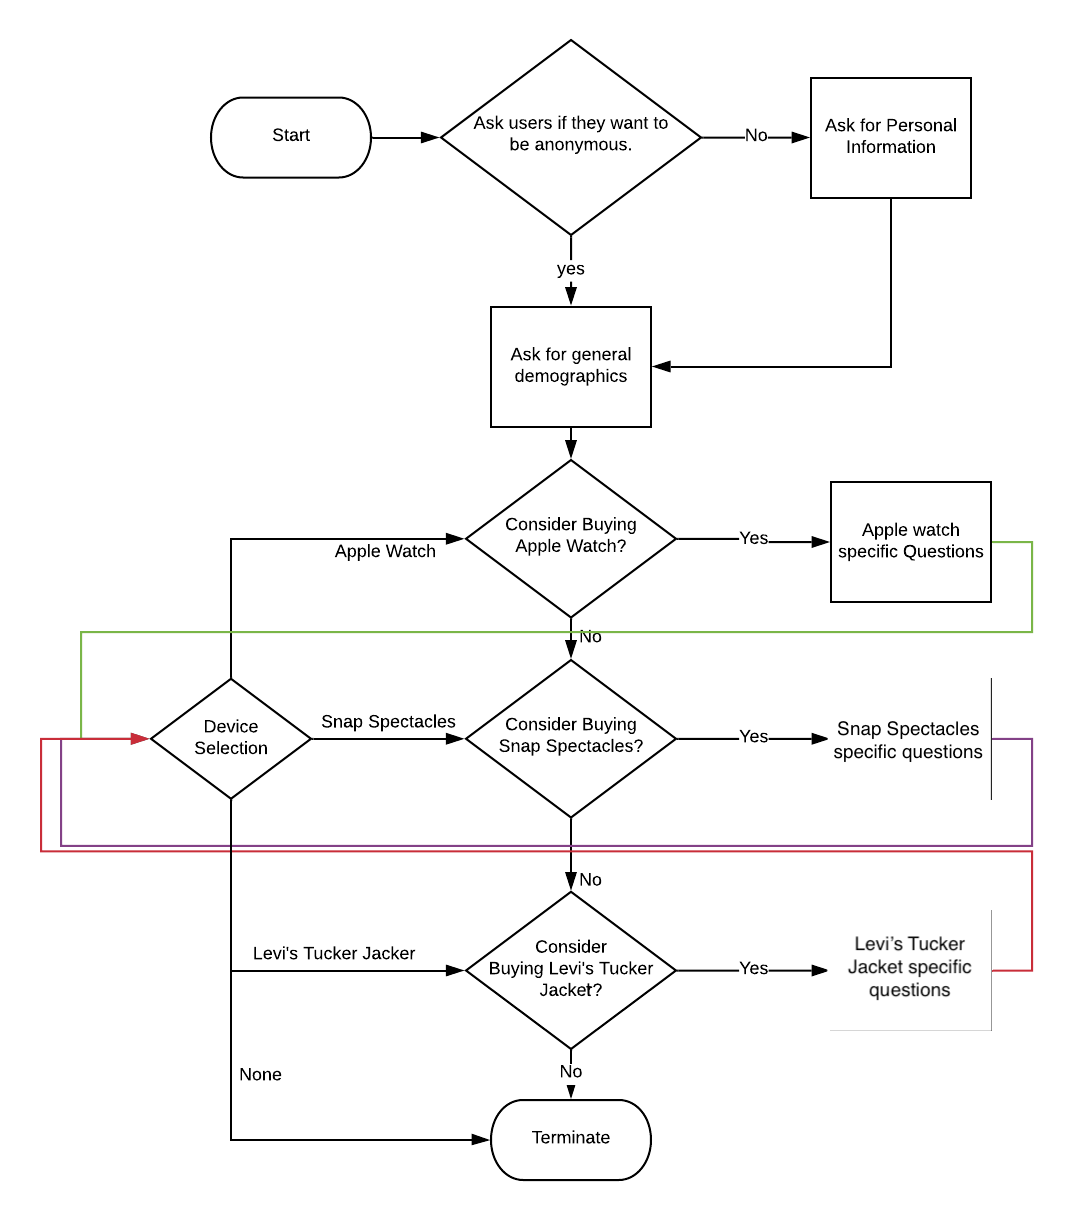
\includegraphics[width=\linewidth]{Flowchart_privacyProject.png}
  \caption{Survey Design Flowchart}
  \label{flowchart}
  \Description{Survey Design Flowchart}
\end{figure}

\section{Analysis}

\subsection{Apple} \label{appleAnalysis}

The majority of the responses were for Apple Watch; around 30 people responded for this part of the survey. There were a total of five questions that were designed to gauge the privacy awareness level amongst the participants. The questions were linked directly to Apple’s privacy policy. A few topics that the questions covered revolved around the topic of permanent deletion of data, reset of digital fingerprint, limiting ad-tracking, and Apple profiling users based on the data they collect. 

For the question “Do you think you can ask Apple to delete the data collected from you permanently?” about \textbf{26\%} of the participants thought they could whereas Apple provides easy steps to delete all the data that was collected from the devices. This information though explicitly mentioned in the Privacy Policy, is never shown during the initial setup of the Apple Watch, or for that matter, any Apple product. If the users had been aware of this information, they could decide for themselves how to control the data. 

For the question “Do you think Apple provides a way to limit ad-tracking for Apple Watch?” around \textbf{40\%} of the participants thought they could. We hypothesize the increase in awareness for this question because Apple gives this option in the Privacy settings of the Watch, iPhone, and other Apple products. Participants are more likely to find information that they have easy access to, rather than the information they have to search for like the previous question. 

\begin{figure}[h]
  \centering
  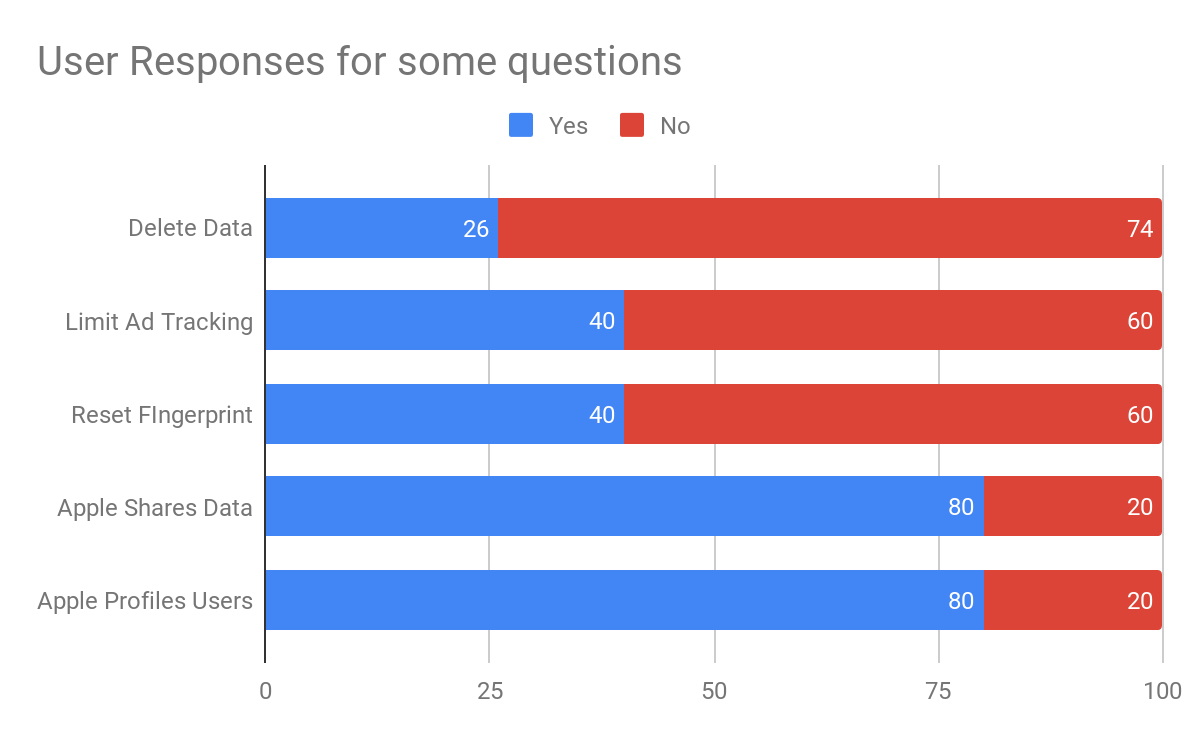
\includegraphics[width=\linewidth]{00-chart.png}
  \caption{User Responses}
  \Description{User Responses}
\end{figure}

For the question “Do you think you can reset your digital fingerprint generated for your Apple Watch?” roughly \textbf{40\%} of the participants answered in the affirmative. The number is similar to the previous question as the two options are on the same page, so we hypothesize that the people answered in the positive for the previous question are the same people who answered this question correctly. 

Finally, we asked two questions that asked about the participants' perspective on whether Apple shares the user’s data for marketing purposes or uses the data to profile the users. Around \textbf{80\%} of the participants answered in the positive. According to the privacy policy, Apple doesn’t. We hypothesize this high positive response is because of the general norm that companies usually follow about data sharing practices. We say the general norm because \textbf{60\%} of the participants out of the \textbf{60\%} had not taken the privacy course with us. 

\begin{figure}[h]
  \centering
  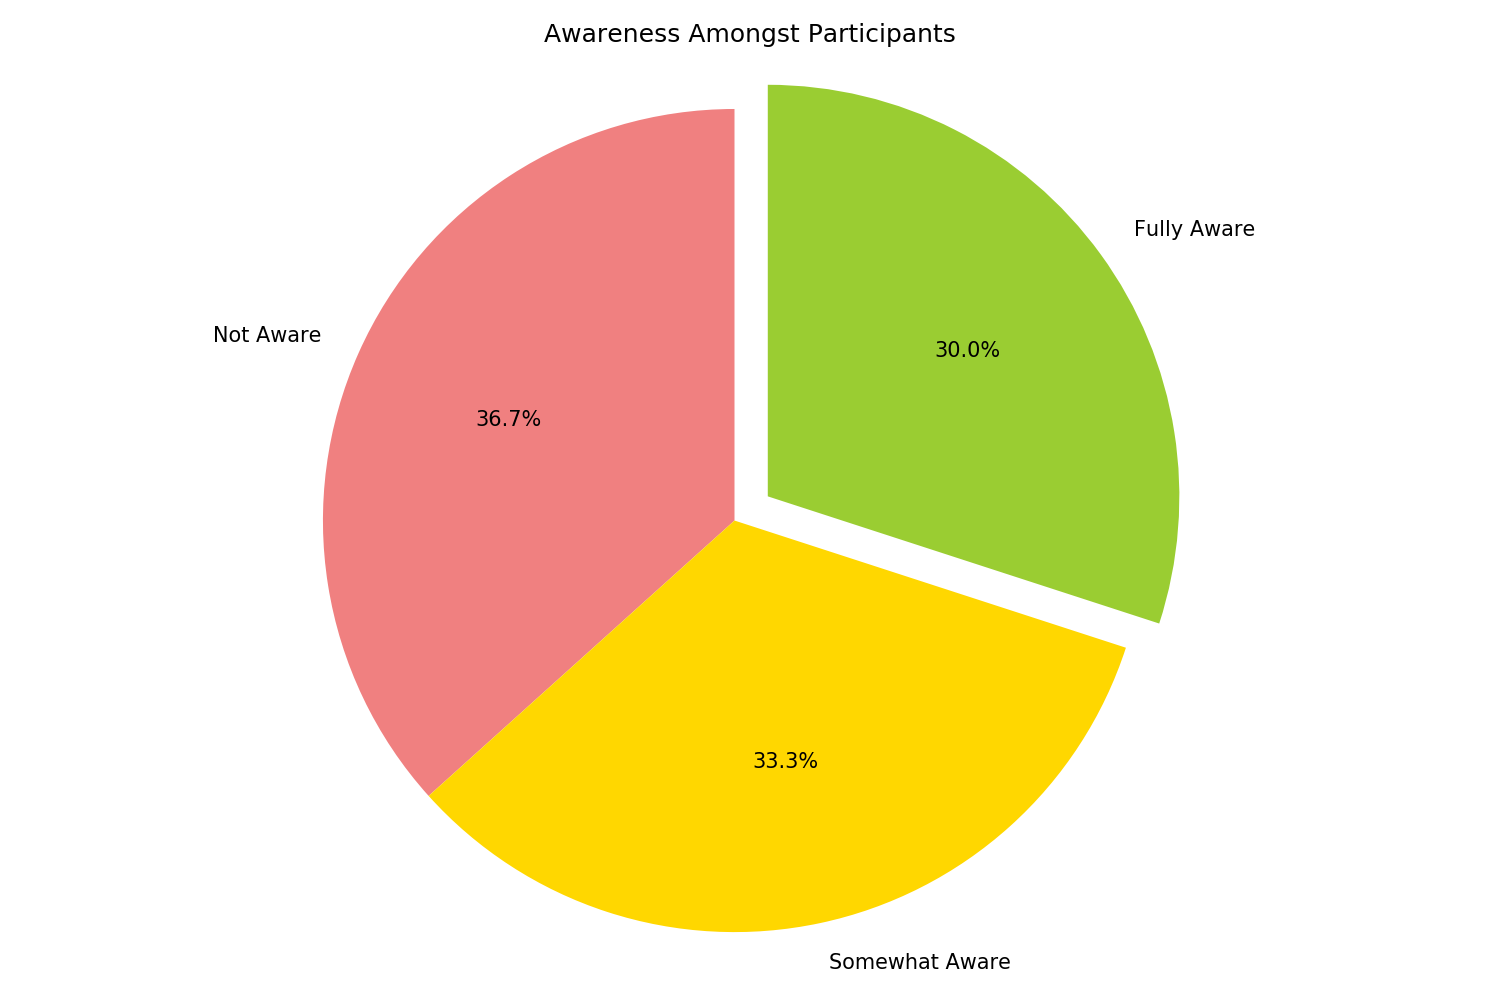
\includegraphics[width=\linewidth]{01-AwarenessAmongstParticipants-Apple.png}
  \caption{Participant Awareness}
  \Description{Participant Awareness}
\end{figure}

Amongst our participants \textbf{50\%} already owned an Apple watch. So we first focus on the remainder of the \textbf{50\%} participants. At the beginning of the study, we hypothesized that knowing with an increase in user awareness, people might change their perspective about buying a product. According to our survey, our hypothesis was correct. Around \textbf{73\%} of the participants changed their perspective from not buying to buying. Whereas the remaining \textbf{27\%} did not change their perspective. Of the people who already owned an Apple watch, \textbf{60\%} participants stated that they did not change their perspective, whereas \textbf{40\%} participants stated that they changed their opinion about owning an Apple Watch. From the data available, we cannot make any conclusive statement as to what they would be doing with their apple watch. Around \textbf{90\%} of the participants thought the information provided in the survey was useful, and that they would better use this information to protect themselves in the future.

In Fig \ref{fig:change} on page \pageref{fig:change}, we see a correlation matrix we see that for the questions for which we had the least user awareness, are the questions for which we see a higher correlation between that question and the reason for the change in perspective. The questions that are highlighted are the questions for profiling users and apple sharing users' data for marketing purposes. We see a little to no correlation for the question which involved limiting ad tracking and resetting digital fingerprint, though there is some correlation, we hypothesize that is because almost \textbf{60\%} of the users cumulatively were aware of that feature, or thought that it was possible. Although correlation is not causation in all cases, the data, in this case, does tip the scale in the other direction.

\begin{figure}[h]
  \centering
  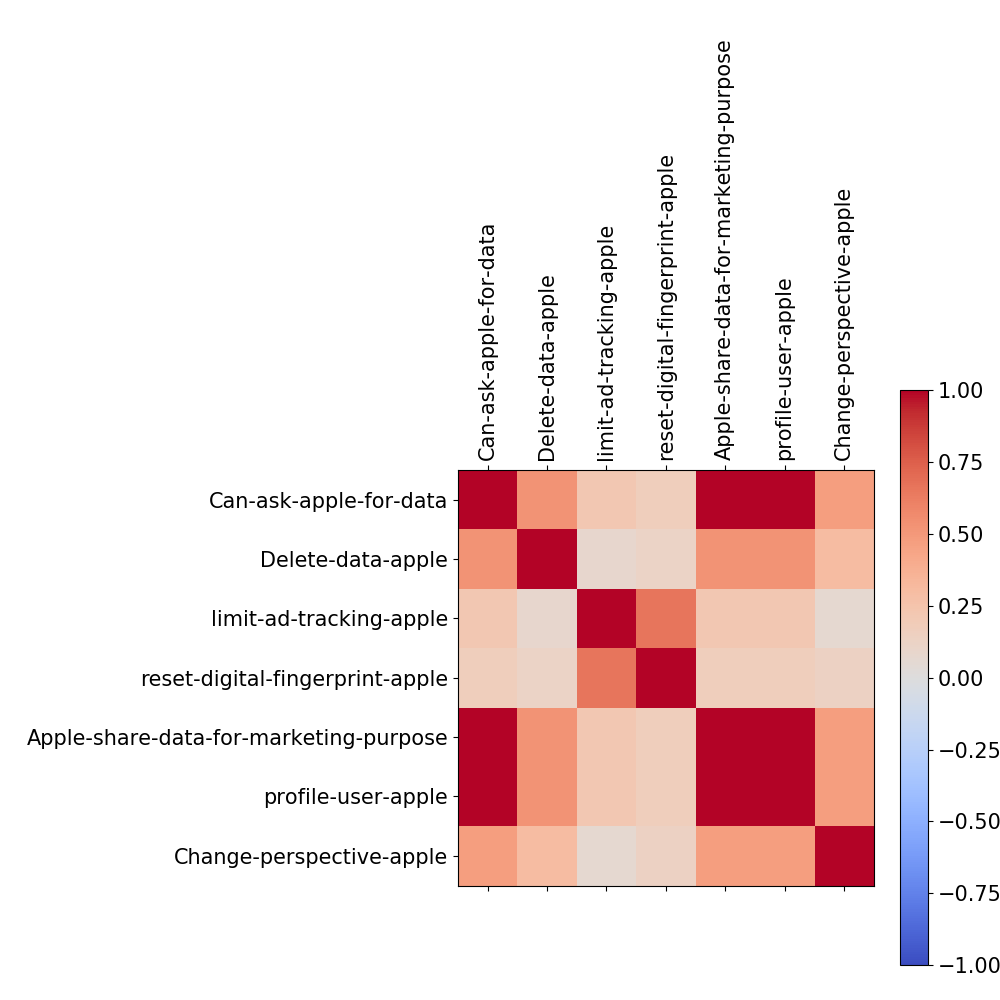
\includegraphics[width=\linewidth]{05-changePerspective-1.png}
  \caption{Correlation matrix for change of perspective}
  \label{fig:change}
  \Description{Change of perception}
\end{figure}

In Fig \ref{fig:changeDos} on page \pageref{fig:changeDos}, we see a similar trend, as in the previous one. The categories for Call-logs, Photos, and Videos have a slightly positive correlation because the majority of the participants thought those data-points are collected. In contrast, according to the privacy policy, Apple does not collect this information. So the absence of it is taken as a positive aspect leading to change in the perspective of the participants from not buying an Apple watch to buying it. For both Location and Voice Recordings, only \textbf{50\%} of the people thought that information is collected. Hence we see the slight negative correlation, which could be because as people who care more about their privacy would change their opinion on seeing that Voice recordings and Location information are being collected. However, this is negated by the fact that Apple claims it does not share this information with third parties. Hence we see the overall increase in the change of opinion, which stems from the awareness of the fact. We see a positive correlation for the fact that Health and Fitness data is collected, which could be because people assume that since its health tracking device, it is justified that Apple collects this data. Moreover, it is later made aware to the users that the Health Data is not shared with Apple until explicitly shared with Apple via either the Health App or the Research App. 

\begin{figure}[h]
  \centering
  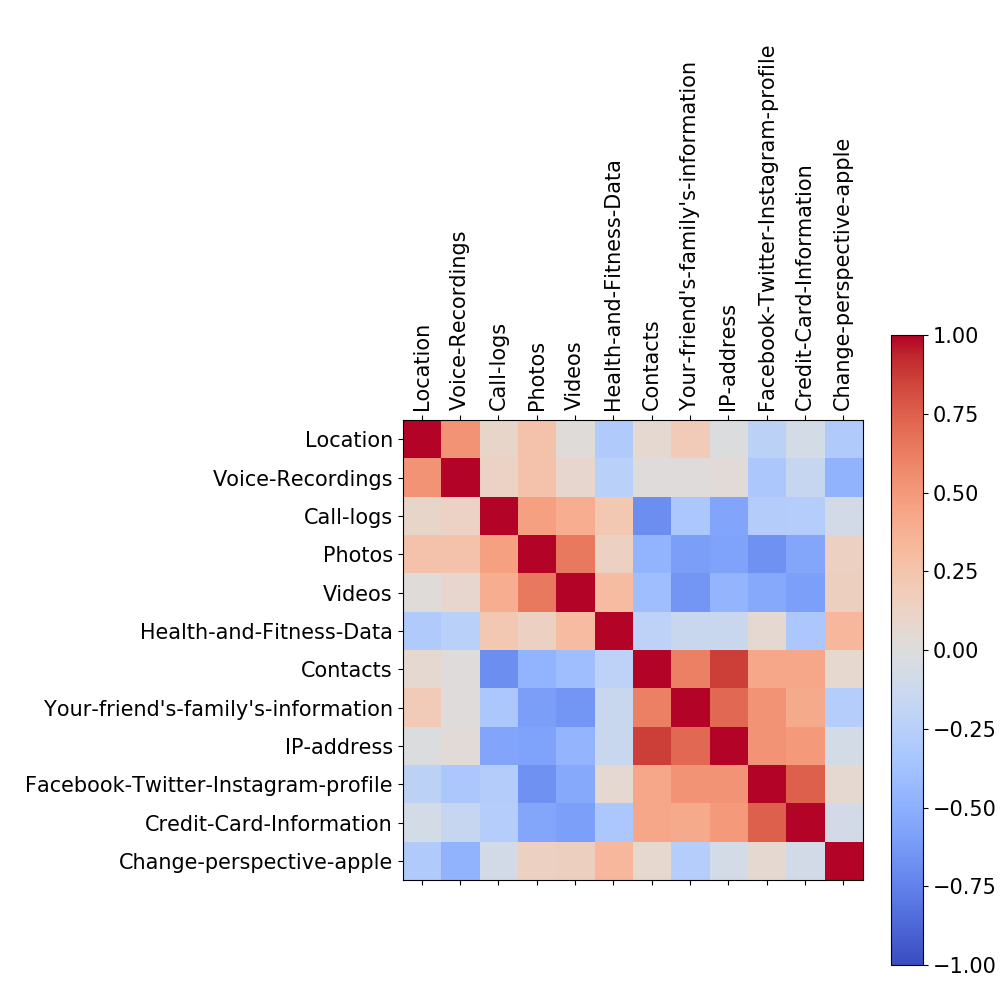
\includegraphics[width=\linewidth]{06-changePerspective-2.png}
  \caption{Correlation matrix for change of perspective}
  \label{fig:changeDos}
  \Description{Change of perception}
\end{figure}


We also carried out another survey that gauged people into different categories, according to Westin’s index. While deciding which questions to ask in the survey, we wanted to revolve around the theme of the Westin’s survey and thus asked questions that had a ”Linear-Scale” in which people could answer. Moreover, having read the Apple’s privacy policy, we had noticed that many businesses do not provide a way to delete the data collected, so we wanted to gather user sentiment on that aspect as well. We also wanted to understand whether different users have a different outlook towards sharing data with health care institutions that use health data for health studies and advertisers that use the data for digital marketing.

\begin{figure}[h]
  \centering
  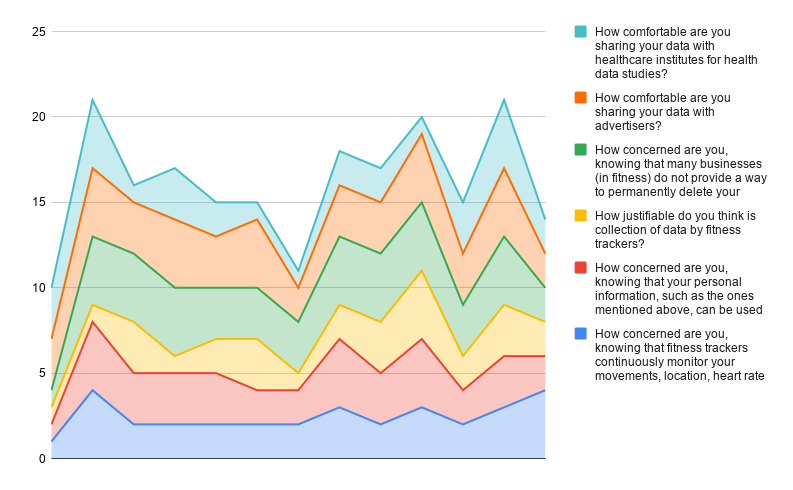
\includegraphics[width=\linewidth]{07-chart2.png}
  \caption{Responses from second survey}
  \label{fig:responses}
  \Description{Responses from second survey}
\end{figure}


15 people replied to the survey. \textbf{60\%} of which do not own a fitness tracker. \textbf{60\%} of the participants that own a fitness tracker were concerned that the fitness trackers track locations, and the data can be harnessed for targeted advertisements. \textbf{40\%} of the people who don’t own a fitness tracker suggest that they don’t find it justifiable for the businesses to store health data.

\textbf{80\%} of the people are concerned that businesses don’t provide a way to delete user’s data permanently. And \textbf{85\%} of the participants are uncomfortable sharing their data with advertisers, but \textbf{60\%} are comfortable sharing with health institutions for health data studies.

From the data that was collected approximately \textbf{40\%} were fundamentalist, \textbf{33\%} were pragmatists and \textbf{27\%} of the participants were unconcerned. We believe the number of unconcerned participants is relatively low because of the age of the participants, which was relatively young.

\begin{figure}[h]
  \centering
  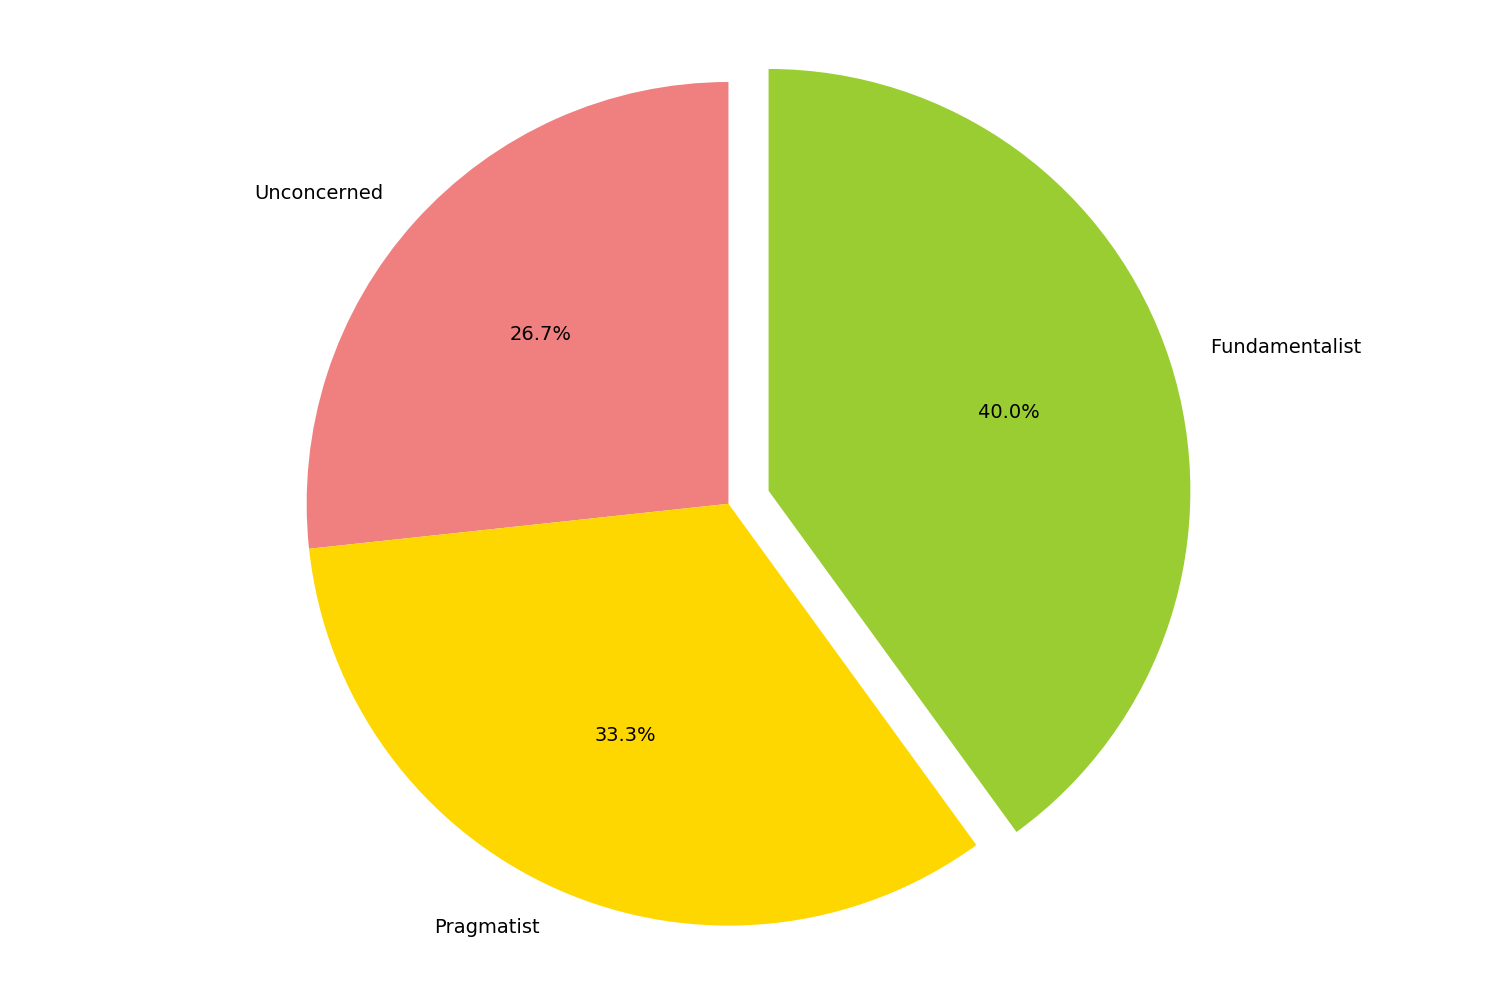
\includegraphics[width=\linewidth]{09-chart.png}
  \caption{Classifying users into group}
  \label{fig:responsesSecondSurvey}
  \Description{Responses from second survey}
\end{figure}


\subsection{Snap Spectacles} \label{snapchatAnalysis}

Snap Spectacles are spectacles that allow the user to record short bursts of video, click images, apply filters, and share them with their social network via the Snap application on their smartphone. They also display a ring of light while recording to indicate to other users that the wearer is currently recording a video. This line of products is relatively new, and hence most users were not aware of the features of this product, the privacy risks posed by it, the types and manner in which data was being collected, etc. This section of the survey specifically received 8 responses. The questions in this section of the survey covered topics such as data collection and sharing policies, privacy and encryption policies, user knowledge about what types of data could be collected at what times, data deletion policies, etc. 

\begin{figure}[h]
  \centering
  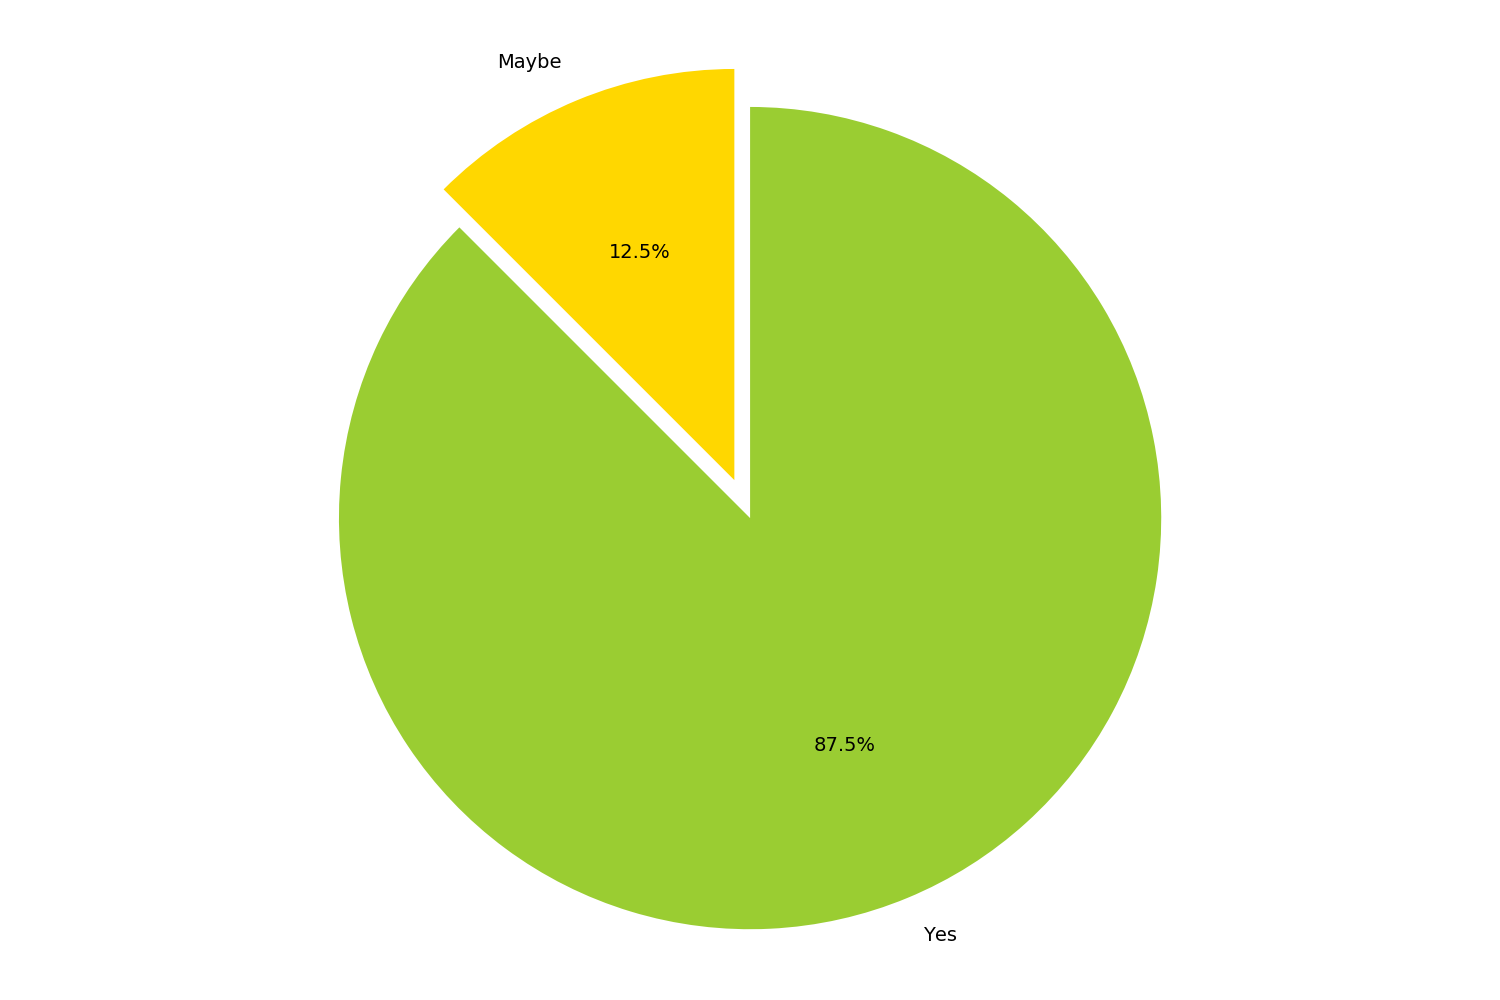
\includegraphics[width=\linewidth]{snap_data_collect.png}
  \caption{Do you think Snap collects data from your Spectacles?}
  \label{fig:snap_data_collect}
  \Description{}
\end{figure}

For the first question in the Snap section of the survey, "Do you think Snap collects data from your Spectacles?" an overwhelming \textbf{88\%} users thought in the affirmative. This shows that respondents of the survey are acutely aware of data collection by the company in some form, and understand that there might be some form of privacy risk associated with it. It is also important to note that, the remaining \textbf{12\%} users answered the question as \textit{"Maybe"} instead of \textit{"No"}. Thus, no user thought that the product did not collect or share any data at all. This might also be indicative of low trust in social media companies due to current events. 

There was also an additional question along the same lines as the previous one. This question asked whether users knew that they could ask Snap to view and download their data. About \textbf{75\%} users answered in the affirmative, which confirms our understanding that respondents were aware of the fact that Snap was collecting data and that they could choose to download and view it. One of the conclusions that can be derived from these two questions is that users were generally aware that Spectacles collect user data, and all data collected by Snap was accessible to the user if needed. 

\begin{figure}[h]
  \centering
  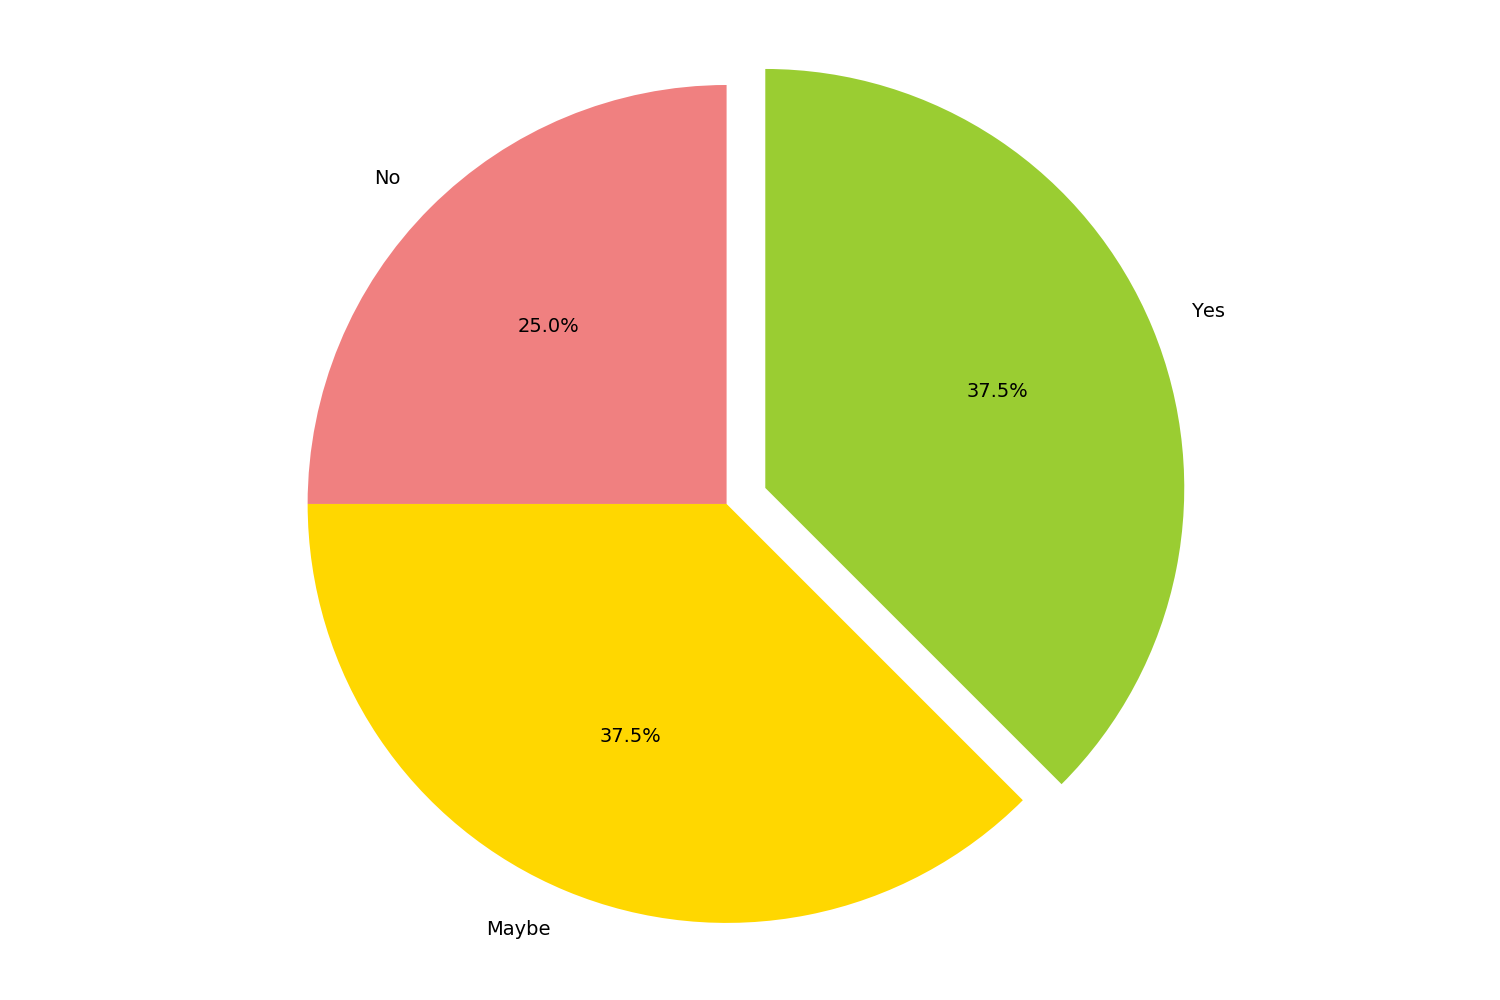
\includegraphics[width=\linewidth]{snap_collect_after_delete.png}
  \caption{Do you think Snap stores your information even after you've deleted your account?}
  \label{fig:snap_data_collect}
  \Description{}
\end{figure}

Another question in the survey that revealed some significant findings was the question, "Do you think Snap stores your information even after you've deleted your account?". Although respondents' opinions were divided in this survey, a majority of them, namely \textbf{62.5\%} users thought that Snap either did not store information after account deletion or was unsure. This was in alignment with the official policy \cite{snap-policy}. The Snap privacy policy \cite{snap-policy} also does not clearly explain the steps that will be taken to erase the data for an account that has been deleted. 

\begin{figure}[h]
  \centering
  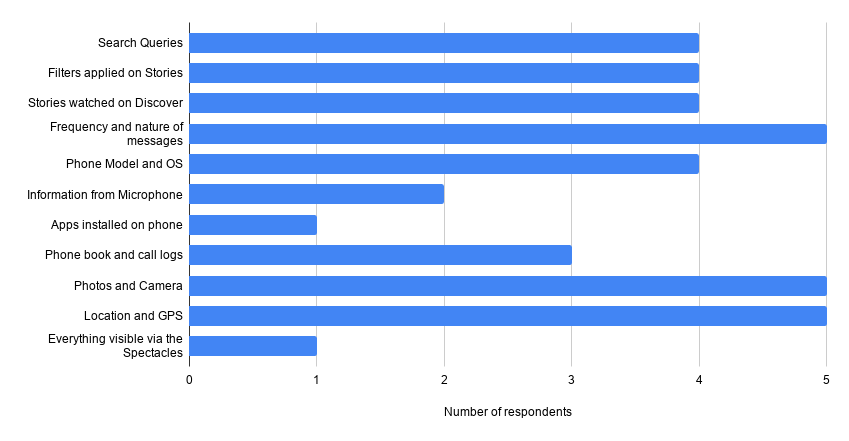
\includegraphics[height=5cm,width=\linewidth]{snap_data_type.png}
  \caption{Types of data collected by Snap}
  \label{fig:snap_data_collect}
  \Description{}
\end{figure}

For the question "What types of data do you think Snap collects?", a large number of respondents (greater than five) were able to correctly answer the most commonly collected types of data such as photos and video, location services and the frequency and nature of messages with friends. However, only one respondent knew that they were also collecting information on how many and which apps are installed on a particular user's phone. It is also surprising that only two respondents knew that Snap could also collect data from their microphone despite it primarily being a videos oriented app. Some of the respondents knew that Snap was also collecting information on phone contacts and logs, user search queries, filters applied on Stories, and the model of the smartphone used by them. In general, we can say that while users were aware of standard data collection practices, they were acutely unaware of many auxiliary ways in which Spectacles were collecting data. 

Additionally, two other questions further strengthened our analysis that users had low awareness about data storage and privacy policies of Snap. In a question that asked whether the respondents knew if they could reset their digital fingerprint with Snap, \textbf{50\%} users answered in the negative and an additional \textbf{12.5\%} users were unsure. In stark contrast to user understanding, this is achievable via the Snap privacy center. In another question that asked whether users thought that Snap could record image data even when the wearer was not actively recording, \textbf{62.5\%} users answered either in the affirmative or were unsure. This is not possible as the Spectacles only record images from the camera when the wearer is actively recording a Story. It is also visible to the people in the vicinity of the wearer as a ring of light is visible in the rim of the Spectacles whenever images or videos are being captured.    

\begin{figure}[h]
  \centering
  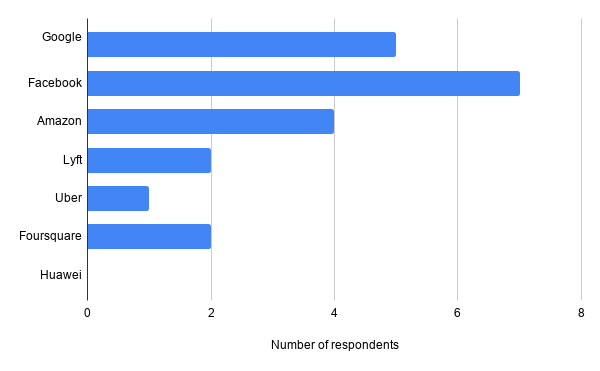
\includegraphics[height=5cm,width=\linewidth]{snap_companies.png}
  \caption{Companies which can access data through services offered by Snap according to respondents}
  \label{fig:snap_data_collect}
  \Description{}
\end{figure}

Since the goal of our study was to analyze whether the user perspective would change if they knew more about the data collection policies of a particular product, we decided to test our respondents' knowledge of the data sharing practices adopted by Snap and then inform them of the correct policies. One of our questions asked respondents to mark all companies who they thought had access to their Spectacles data. \textbf{87.5\%} users thought that Snap shared data with Facebook, and \textbf{62.5\%} users thought Snap also shared data with Google. According to Snap's privacy policy \cite{snap-policy}, they do not share data with Facebook, but they do share location and advertisement data with Google. These results are not surprising as a lot of their previously unknown data collection policies have been highlighted \cite{facebookdatashare} in the media in recent days. Thus users could have speculated that Facebook also has access to advertisement data via Snap, among other sources.

On the other hand, only \textbf{12.5\%} users thought that Snap shared its location data with Uber Inc and another \textbf{25\%} thought that they shared location data with Lyft. According to the privacy policy of Snap \cite{snap-policy}, both of these are true. Thus, we can see that users were ill-informed about the data-sharing practices adopted by Snap, and had little knowledge of which specific companies had access to what type of data via the Snapchat app.

\begin{figure}[h]
  \centering
  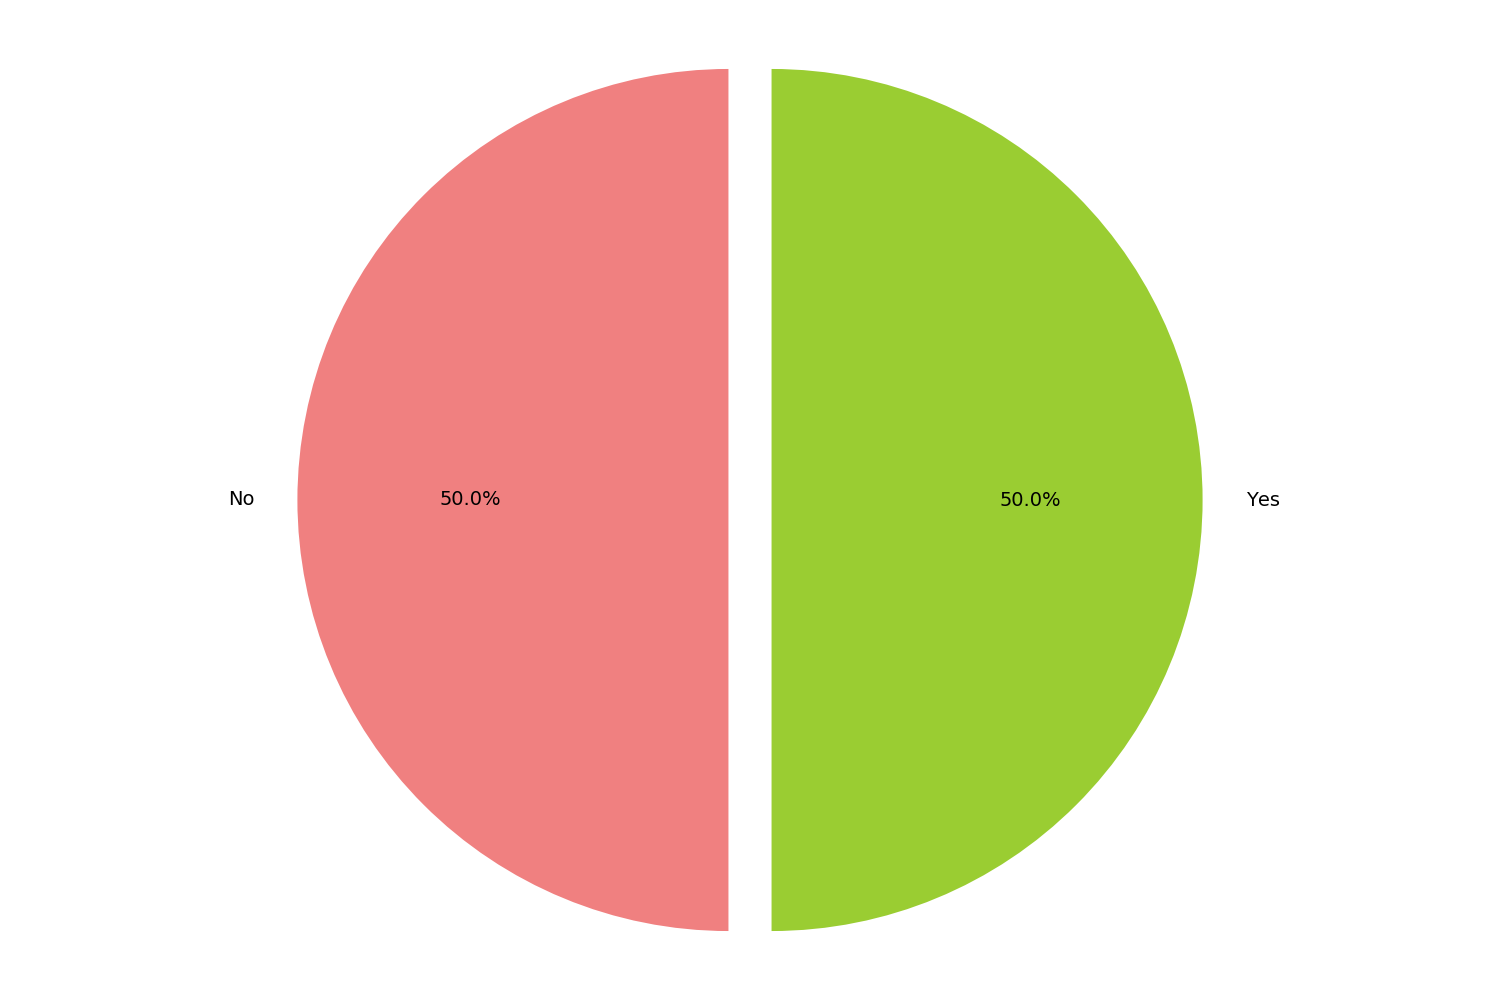
\includegraphics[width=\linewidth]{snap_change_perspective.png}
  \caption{Does knowing this information change your mind about buying Snap spectacles?}
  \label{fig:snap_data_collect}
  \Description{}
\end{figure}

At the end of the Snap Spectacles section, we asked the respondent if knowing the information that they had just learned changed their minds towards buying the product. \textbf{50\%} users responded in the affirmative to this question. This signifies that a medium to a high volume of users changed their perspective towards buying the Snap Spectacles after they were introduced to all the data collection, storage, and sharing practices adopted by Snap. These users were unaware of the specific companies that had access to their data, the "hidden" types of data that were being collected, and the amount of time for which their information was stored even after they had deleted their account.  

\subsection{Levi's} \label{levisAnalysis}

Lorem ipsum dolor sit amet, consectetur adipiscing elit. Morbi
malesuada, quam in pulvinar varius, metus nunc fermentum urna, id
sollicitudin purus odio sit amet enim. Aliquam ullamcorper eu ipsum
vel mollis. Curabitur quis dictum nisl. Phasellus vel semper risus, et
lacinia dolor. Integer ultricies commodo sem nec semper.


\section{Limitation and Future Work} \label{limitationAndFutureWork}
A limitation of the study was that we never created any Personas for the people who could potentially be part of the survey. The survey could have been more focused. The current study gives some correlation between the variables collected, as shown in section \textbf{\ref{appleAnalysis}} on page \textbf{\pageref{fig:changeDos}}. To provide a stronger correlation between the different variables, additional information would be needed. The additional information would be to map the factors responsible for influencing the decision of the users.  

Using this additional information a focus group can be used to understand if a product with all the variables with the highest correlation when put together would be a product that would be preferred over other products.


\bibliographystyle{ACM-Reference-Format}
\bibliography{sample-base}


\end{document}
\endinput
%%
%% End of file `sample-sigconf.tex'.
